\documentclass{article}
\usepackage{graphicx}
\usepackage{booktabs}
\usepackage{amsmath}
\usepackage[margin=1in]{geometry}
\usepackage{hyperref}

\title{Heart Disease Prediction using PCA, Naive Bayes and Decision Trees}
\author{Eric Iov}
\date{June 2026}

\begin{document}

\maketitle

\begin{abstract}
% TODO: fill in after all steps are done (2-3 paragraphs)
\end{abstract}

\section{Introduction}
% TODO: fill in — problem description, motivation, state of the art references, brief solution overview

\section{Description of the Dataset}

The Cleveland Heart Disease dataset was obtained from the UCI Machine Learning Repository \cite{uci}. It contains 303 records and 13 features, along with a binary target variable indicating the presence (1) or absence (0) of heart disease. The target was derived by binarizing the original ordinal variable (values 0–4), where any value greater than 0 was mapped to 1.

\subsection*{Features}

The dataset includes a mix of continuous and categorical attributes:

\begin{itemize}
    \item \textbf{Continuous:} age, trestbps (resting blood pressure), chol (serum cholesterol), thalach (maximum heart rate), oldpeak (ST depression)
    \item \textbf{Binary:} sex, fbs (fasting blood sugar $>$ 120 mg/dl), exang (exercise-induced angina)
    \item \textbf{Categorical:} cp (chest pain type), restecg (resting ECG results), slope (slope of peak exercise ST segment), ca (number of major vessels), thal (thalassemia type)
\end{itemize}

\subsection*{Statistical Summary}

Key statistics for the continuous features are summarized below:

\begin{table}[h]
\centering
\begin{tabular}{lcccc}
\toprule
Feature & Mean & Std & Min & Max \\
\midrule
age       & 54.44 & 9.04  & 29  & 77  \\
trestbps  & 131.69 & 17.60 & 94  & 200 \\
chol      & 246.69 & 51.78 & 126 & 564 \\
thalach   & 149.61 & 22.88 & 71  & 202 \\
oldpeak   & 1.04  & 1.16  & 0.0 & 6.2 \\
\bottomrule
\end{tabular}
\caption{Statistical summary of continuous features}
\end{table}

\subsection*{Missing Values}

The dataset contains 6 missing values in total: 4 in the \texttt{ca} column and 2 in the \texttt{thal} column, representing approximately 2\% of the data. All other features are complete.

\subsection*{Class Distribution}

The dataset is slightly imbalanced: 164 records (54.1\%) belong to the negative class (no disease) and 139 records (45.9\%) to the positive class (disease), as shown in Figure \ref{fig:class_dist}. The imbalance is mild and does not require special resampling techniques.

\begin{figure}[h]
    \centering
    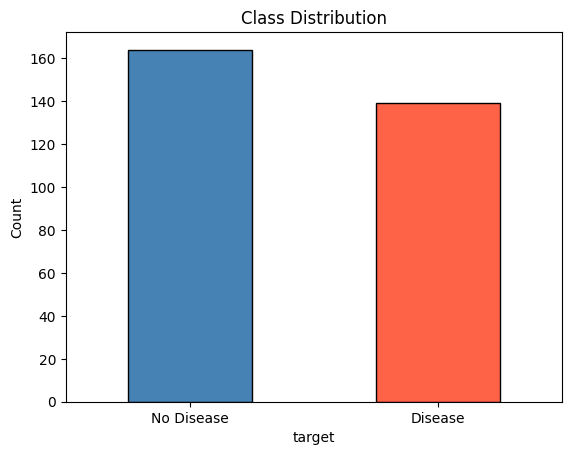
\includegraphics[width=0.5\textwidth]{class_distribution.png}
    \caption{Class distribution of the target variable}
    \label{fig:class_dist}
\end{figure}

\subsection*{Feature Distributions}

The distributions of all features are shown in Figure \ref{fig:hist}. Several features (e.g. \texttt{sex}, \texttt{fbs}, \texttt{exang}) are binary and heavily skewed toward one value. Continuous features such as \texttt{age} and \texttt{chol} follow approximately normal distributions, while \texttt{oldpeak} is right-skewed.

\begin{figure}[h]
    \centering
    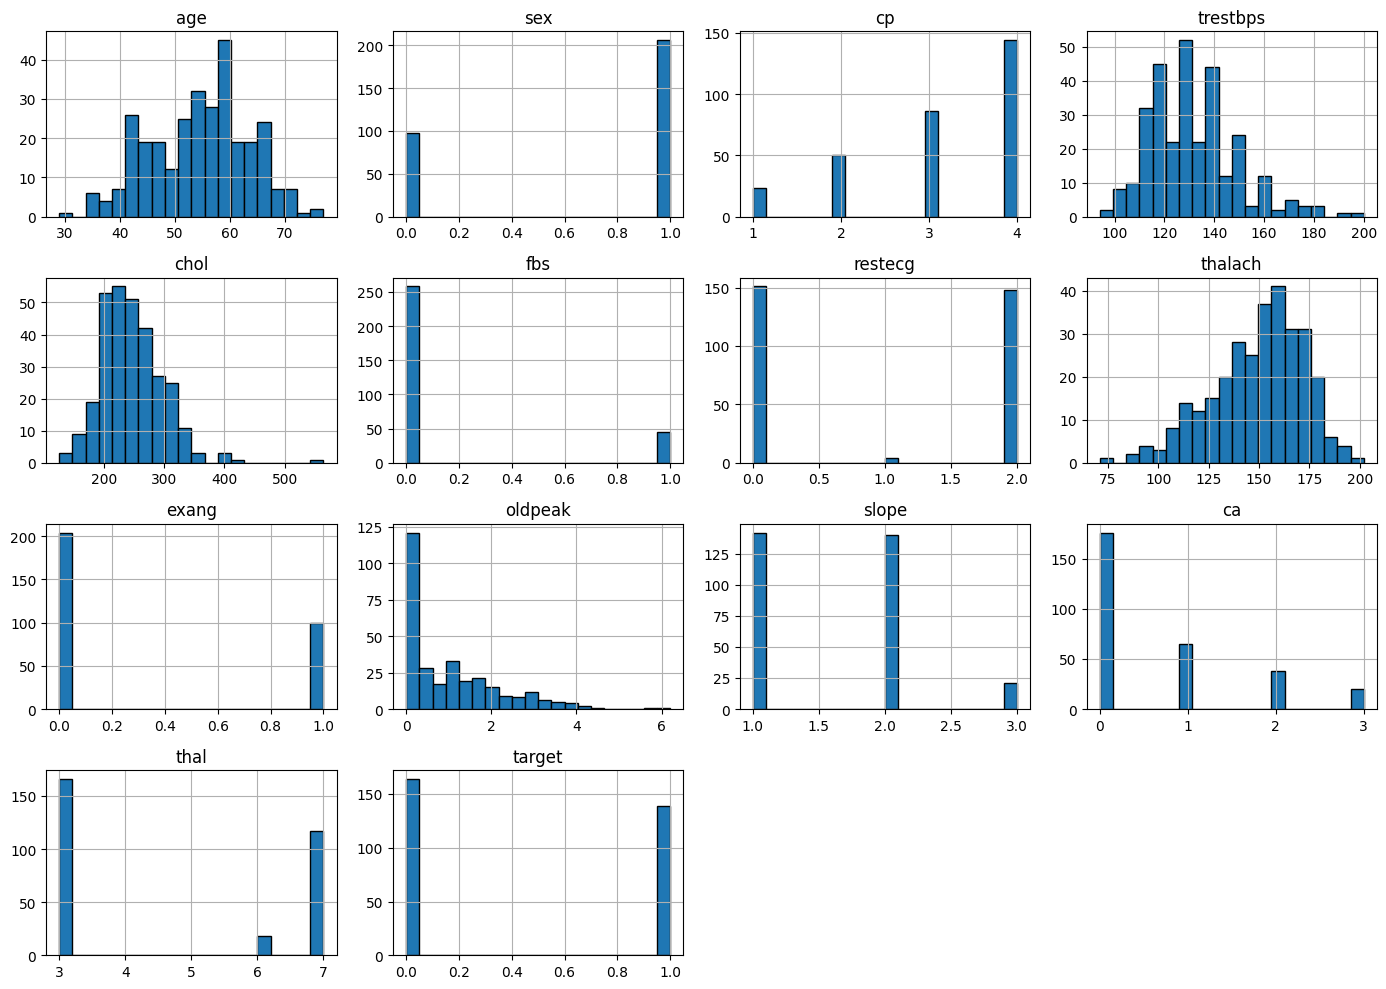
\includegraphics[width=\textwidth]{feature_distributions.png}
    \caption{Distribution of all features}
    \label{fig:hist}
\end{figure}

\subsection*{Correlation Analysis}

The correlation matrix (Figure \ref{fig:corr}) reveals that the features most correlated with the target are \texttt{thal} (0.53), \texttt{ca} (0.46), \texttt{cp} (0.41), \texttt{thalach} (-0.42), and \texttt{exang} (0.43). Features such as \texttt{fbs} and \texttt{restecg} show very low correlation with the target and may contribute less to classification performance.

\begin{figure}[h]
    \centering
    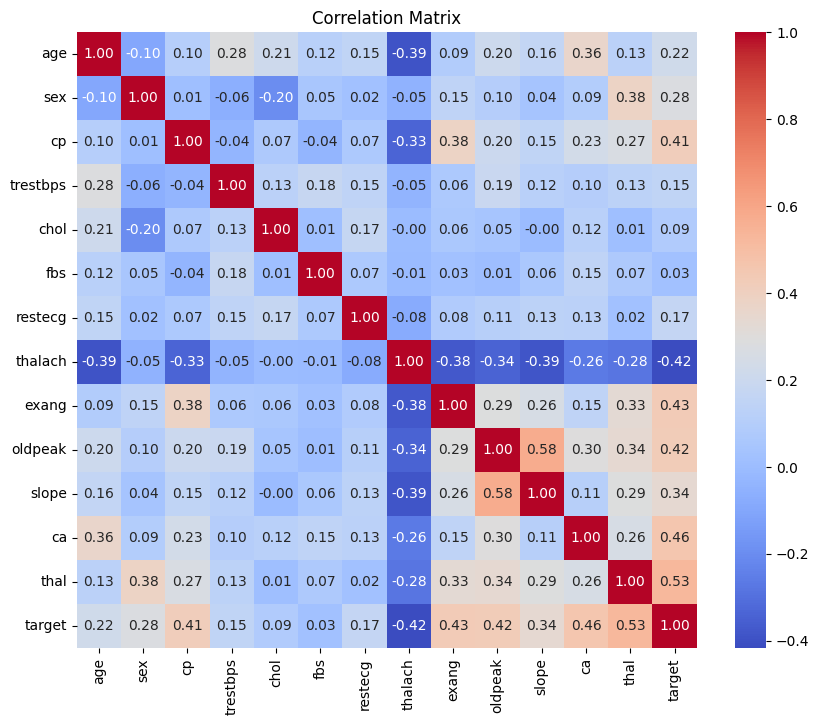
\includegraphics[width=0.8\textwidth]{correlation_matrix.png}
    \caption{Correlation matrix of all features}
    \label{fig:corr}
\end{figure}

\section{Description of the Processing Flow}
% TODO: fill in after Steps 2 and 3

\section{Results}
% TODO: fill in after Steps 4, 5, and 6

\section{Conclusions}
% TODO: fill in after all steps are done

\begin{thebibliography}{9}
\bibitem{uci}
    UCI Machine Learning Repository: Heart Disease Dataset.
    \url{https://archive.ics.uci.edu/ml/datasets/heart+disease}
\end{thebibliography}

\end{document}
